\section{\name Overview} \label{sec:overview}
\subsection{Requirements}\label{sec:req}
Before we describe the design overview, We'd like to share the requirements we considered in the design.
We summarize the requirements as follows, in terms of compatibility, development cost and security.
\begin{enumerate}
\item (R1) Unaltered system security. The new scheme should not sacrifice the system security to obtain benefits from I/O performance. No one likes to use a system with known design loopholes.
\item (R2) Compatible with legacy applications. The new scheme should limit the modifications on the guest kernel and the hypervisor, without any modifications on the existing applications.
\item (R3) Small modifications. The new scheme should minimize the development cost on the guest kernel and the hypervisor.
\item (R4) Minimizing IOTLB flushes. The new scheme should minimize the number of IOTLB flushes, such as reducing the number to zero.
\end{enumerate}

\subsection{Design Rationale}\label{sec:rationale}
It is challenging to reduce the number of the IOTLB
flushes while achieve the above four requirements.
A possible approach is to let the hypervisor to manage the page table in its own space.
In this way, there is no need for flushing IOTLB, but it will dramatically increase the size of the hypervisor, and consequently reduce the system security level.
Another approach is to do the IOTLB flushing in a batch, instead of flushing the IOTLB entry one after another.
This approach retains the system security, but it could not eliminate all IOTLB flushes, only reducing the number of IOTLB flushes to a certain level.
In this paper, we propose a novel approach - \name, which could reduce the number of IOTLB flush to zero only with small modifications on the guest kernel and the hypervisor, without sacrificing the system security.

Specifically, \name creates a page table cache for caching the destructed guest page-table pages.
For the pages in this cache pool, the guest kernel could read and write them, but the DMA requests cannot access them, meaning they are non-readable and non-writable for DMA.
By configuring them in this way, the destructions of the guest page tables will not trigger IOTLB flushes any more, as the permissions for DMA are kept the same.
In addition, the creations of the page table also do not need IOTLB flush as the guest kernel could allocate pages from the cached pool, instead of allocating pages from the slow and inefficient buddy system.

\subsection{Design Rationale}
As can be seen in figure ~\ref{fig:overview}, \name introduces a cache flag to enforce fine-grained access control in order to ensure security without flushing IOTLB. Also, \name proposes a novel cache mechanism to support the access control while facilitate the speed of every level of page table allocation/deallocation, saving CPU time while causing small impacts on memory usage.

\begin{figure}[ht]
\centering
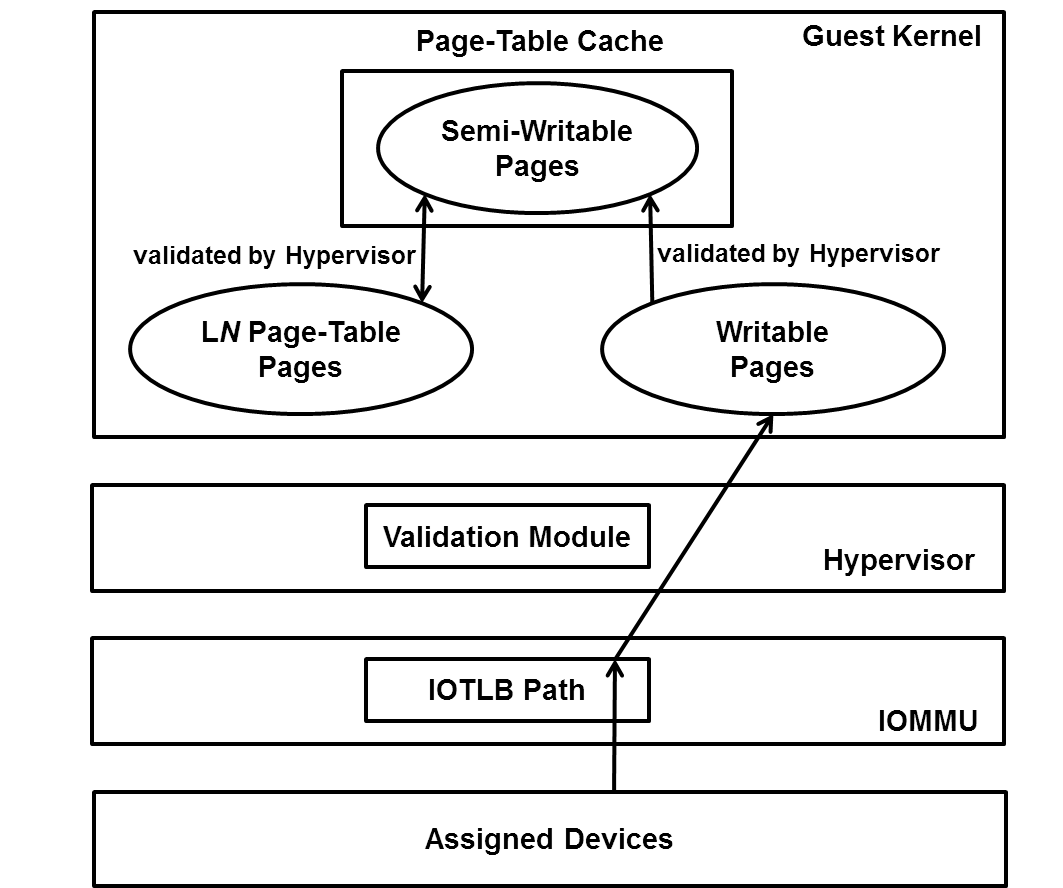
\includegraphics[width=0.5\textwidth]{image/overview/overview.png} \\
\caption{Overview}
\label{fig:overview}
\end{figure}

\subsubsection{Fine-Grained Access Control}
%firstly, talk about how to reduce the IOTLB flush.
As revealed in previous sections, access control to writable pages is at a coarse granularity. Xen allows write-access both for guest OS and assigned I/O devices. Instead, \name caches a certain number of writable pages, prohibits DMA access for the cached writable pages while OS still has its write-permission. If they are updated to be page tables, Xen only limits OS to read-only permission (software protection) without modifying I/O page tables as well as IOTLB. Specifically, Xen maintains a new flag called \textbf{cache} with a machine page (a cached page), indicating that the corresponding page is cached by guest OS and free from DMA-access. Whatever page type a machine page is, if it owns the flag, Xen neither maps nor unmaps it from I/O page tables, thus avoiding an IOTLB-flush. Note that \name only considers page type updates between writable and page-table.

For instance, if guest OS creates a new page-table, Xen firstly reuses the validation process to enforce software protection, and then checks if the page has the \textbf{cache} flag. If so, the only thing that Xen needs to do is to update the page to be a page-table. If not, Xen sets the page with the new flag, clears \emph{read} and \emph{write} permission fields in I/O page tables and flushes IOTLB. As for the guest page table destruction, Xen also reuses existing security checks to remove software protection while maintains DMA prevention, after which the corresponding page is (if without the flag) set with the \textbf{cache} flag and updated to be writable. Figure \ref{fig:cache-flag} describes the process.

\begin{figure}[ht]
\centering
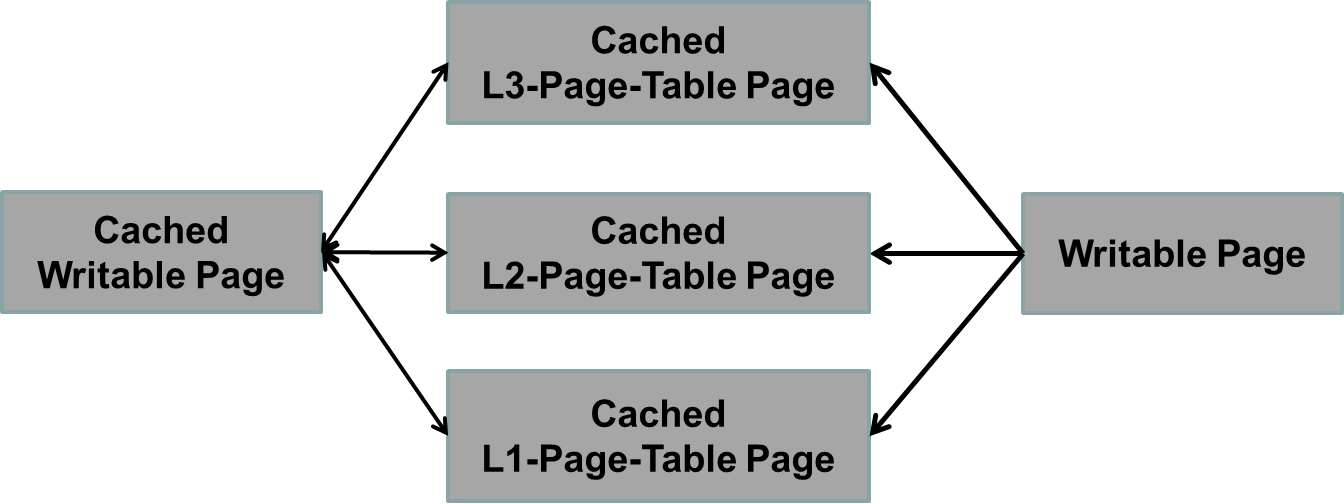
\includegraphics[width=0.5\textwidth]{image/overview/page-type-updates-with-cache-flag.png} \\
\caption{Page Type Updates with Cache Flag}
\label{fig:cache-flag}
\end{figure}

As can be seen in Figure \ref{fig:cache-flag}, every time page type updates between writable and page-table occur, every related page will own the flag, inaccessible to devices and all Xen needs to is to validate guest OS, having protected guest page tables and improved IOTLB performance, which satifies R1,2.

As writable pages with \textbf{cache} flag freed by guest OS cannot be mixed with ordinary pages in the buddy system, \name builds up cache pools to manage freed writable pages in the OS space to function properly and serve as caches of page tables.

\subsection{Cache Mechanism}
%secondly, design the cache pool to support it
If guest OS directly frees pages with cache flag to the buddy system, which may allocate them for DMA transactions. This will lead to unacceptable access faults. As a result, \name enables OS to cache the writable pages for page-tables. Specifically, \name defines new cache allocating and freeing functions for every level of page table to manage cache and whichever existing page-table function will invoke the corresponding cache function. By this approach, \name reserves page-table caches. When dealing with process creation/destruction, OS allocates pages from or frees them into the cache pool instead of the buddy system, reducing time cost, thus meeting R2.

Cache mechanism begins its life-cycle either automatically with system booting up or dynamically during system runtime. \name provides an interface for users to activate dynamically. Utilizing the feature, users can improve system performance in an on-demand way (e.g., too many process-creation at some time). Basically, if the mechanism is activated dynamically, there may exists a few writable pages without cache flag and this does not ruin the security while flush IOTLB only once. Also note that when every cache pool is empty initially or OS asks for more pages (e.g., many processes creations) than cache pool could supply, cache allocating function always requests pages from the buddy system, which also affect IOTLB once.

During the runtime of the cache, \name also needs to control the memory size that caches take up. If the cache size becomes larger, it is necessary for cache freeing function to free pages from the pool into the buddy system. When to free pages in pool depends on two factors, namely $1$) a proportion between pages in use and in pool, and $2$) a total number of pages in use and in pool. If both factors exceed specific thresholds, respectively, corresponding cache flags must be cleared before the pages are freed. Thus, \name defines a new hypercall for OS. When handling the hypercall, Xen mainly clears the flag of specified pages, maps freed pages in the I/O page tables and flushes IOTLB. It can be concluded that inappropriate thresholds will lead to the flushes of IOTLB. Because of that, \name offers an interface for users to modify the default values of both thresholds in order to reduce IOTLB-flush or adjust cache size (meets R2). The default thresholds are determined by conducting experiments where no pages are freed to the buddy system (see details in section~\ref{sec:eva}), and the page number to free is stated in the equation below: $\Delta$num\_to\_free $=$ num\_in\_pool $-$ num\_in\_use. If users have only a few available memory in extreme cases, they are provided with another interface to manually free all pages in cache into the buddy system, thus relieving system's pressure while badly affecting IOTLB. Using the two interfaces, users have full control of the page-table cache.

This is the life-cycle of a cached page, originating from the buddy system, freed into the cache, then maybe allocated by the cache and finally freed into the buddy system when necessary.

Section~\ref{sec:implementation} will demonstrate its small modifications in details.
